\section{Аннотация}
\underline{Цель работы}: 
\begin{enumerate}
    \item Вывести зависимости для колебаний воздуха в духовом инструменте.
    \item Изучить продольные стоячие волны на примере колебаний воздуха.
    \item Проверить справедливость формулы для зависимости частоты от номера гармоники для духовых инструментов.
\end{enumerate} \par
\underline{Оборудование}: 3 Блок-флейты HOHNER, HOHNER и YRS-23 YAMAHA;Большая флейта YFL 212;микрофон FIFINE K669; Программа анализа звука Friture.
\newpage

\section{Теоретические сведения}
\subsection{Колебания воздуха в трубе}
Составим уравнение колебаний газа в трубе. Обозначим координату частиц, находящихся в каком-то поперечном сечении трубы через $x$, а смещение частиц этого сечения вдоль оси трубы при колебаниях через $\xi$. Рассмотрим объем газа в виде цилиндра с площадью основания $S$ и высотой $\Delta х$ (Рисунок \ref{fig:smeshenie}). Масса газа, заключенного в этом объеме, равна $\rho S \Delta x$, где $\rho$ --- плотность газа в покое. Если колебания частиц газа отсутствуют, то давление в сечениях $x$ и $х + \Delta х$ одинаково и равно $p$. При колебаниях смещения $\xi$ частиц с разными $х$ в каждый момент времени оказываются разными. Поэтому рассматриваемый объем деформируется, и давление в разных сечениях цилиндра уже не будет одинаковым. 
Мгновенное значение давления в некотором сечении трубы можно представить в виде:

\begin{wrapfigure}{l}{0.35\textwidth} 
    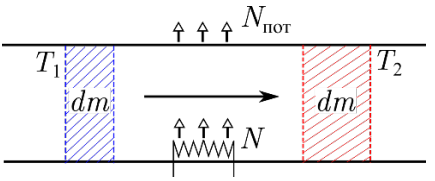
\includegraphics[width=0.35\textwidth]{foto1.png}
    \caption{Смещение газа в трубе}
    \label{fig:smeshenie}
\end{wrapfigure}

$p^{\prime} = p + \Delta p, \Delta p \text{ --- звуковое давление.}$
Ввиду малости $\Delta  х$  проекцию ускорения на ось $x$
для всех точек цилиндра можно считать одинаковой и равной $\dv[2]{\xi}{t}$. Для нахождения проекции на ось $х$ силы, действующей на рассматриваемый объем, нужно взять произведение площади основания цилиндра $S$ на разность давлений $p^{\prime}$ в сечениях $x + \xi$ и $x + \Delta x + \xi + \Delta\xi$:
\begin{equation}
    F_{x} = \left( p^{\prime} (x + \xi) - p^{\prime}(x + \Delta x + \xi + \Delta\xi)\right)S
\end{equation}
Пренебрегая слагаемыми высших порядков малости получаем $F_{x} \approx -S\Delta x \dv{p^{\prime}}{x}, \Delta x \ll \Delta \xi$.\\
Второй закон Ньютона:
\begin{align}
    \rho S \Delta x \dv[2]{\xi}{t} &= -S\Delta x \dv{p^{\prime}}{x} \\
    \rho\dv[2]{\xi}{t} &= -\dv{p^{\prime}}{x}
\end{align}

Получаем дифференциальное уравнение:
\begin{equation}
    \rho\dv[2]{\xi}{t} = -\dv{p^{\prime}}{x}    
\end{equation}

в котором две неизвестные функции $\xi$ и $p^{\prime}$. Выразим одну из этих функций через другую. При колебаниях в трубе сжатия и разрежения газа следуют друг за другом так часто, что смежные участки среды не успевают обмениваться теплом, и процесс можно считать адиабатическим. При адиабатическом процессе связь между давлением и объемом газа задается уравнением:
\begin{align}
    pV^{\gamma} = const,
\end{align}
где $\gamma$ --- отношение теплоемкости при постоянном давлении к теплоемкости при постоянном объеме.

В соответствии с этим уравнением получаем:
\begin{equation}
    p(S\Delta x)^{\gamma} = p^{\prime}\left[ S(\Delta x + \Delta \xi)\right]^{\gamma} = p^{\prime}\left[ S \left(\Delta x + \dv{\xi}{x}\Delta x\right) \right]^{\gamma} = p^{\prime}(S \Delta x)^{\gamma} \left( 1 + \dv{\xi}{x}\right)^{\gamma},
\end{equation}

где $p$ --- давление газа в покое.\\
Сократим на $(S \Delta x)^{\gamma}$ и разложив выражение $\left( 1 + \dv{\xi}{x}\right)^{\gamma}$ по степеням $\dv{\xi}{x}$ и считая, что $\dv{\xi}{x} \ll 1$ и пренебрегая членами высших порядков малости получаем:
\begin{align}
    p &= p^{\prime} \left( 1 + \gamma \dv{\xi}{x} \right) \\
    p^{\prime} &= \frac{p}{1 + \gamma \dv{\xi}{x}} \approx p \left( 1 - \gamma \dv{\xi}{x}\right).
\end{align}
Получаем $\frac{p^{\prime} - p}{p} = -\gamma \dv{\xi}{x}$.\\
Так как $\gamma$ порядка единицы, то $\mid \dv{\xi}{x} \mid \approx \mid 
\frac{\Delta p}{p} \mid \ll 1$ --- отклонение давления от среднего много меньше самого давления (атмосферное давление 760 мм. рт. ст., а амплитуда колебания воздуха не превышает 1 мм. рт. ст.).\\
Продифференцировав по x, получаем
\begin{equation}
    \dv{p^{\prime}}{x} = -\gamma p \dv[2]{\xi}{x}
\end{equation}
Подставляя это выражение в дифференциальное уравнение, получаем уравнение колебаний смещения $\xi$ в трубе с газом при адиабатическом законе
\begin{equation} \label{eq:volnovoe_uravnenie}
    \dv[2]{\xi}{t} = c^{2}\dv[2]{\xi}{x}
\end{equation}
где $c = \sqrt{\gamma \frac{p}{\rho}}$ --- скорость распространения колебаний (скорость звука).

Так как при атмосферном давлении и обычных температурах большинство газов по своим свойствам близки к идеальному, то используя уравнение Менделеева-Клапейрона, получим для скорости звука формулу
\begin{equation}
    c = \sqrt{\frac{\gamma R T}{M}}
\end{equation}
Уравнение \ref{eq:volnovoe_uravnenie}  называется волновым. Частным решением уравнения \ref{eq:volnovoe_uravnenie}  является бегущая волна вдоль оси $x$
\begin{equation}
    \xi = A cos(\omega t - kx + \varphi),
\end{equation}\\
где $\omega$ --- циклическая частота колебаний, $k = \frac{\omega}{c}$ --- волновое число, $\varphi$ --- начальная фаза.\\ 
Волна бегущая навстречу описывается уравнением $\xi = A cos(\omega t - kx + \varphi)$.\\
Волна, бегущая вдоль трубы будет отражаться от конца, а закон ее отражения определяется физическими условиями на конце.\\
В нашем случае с духовыми инструментами оба конца открыты, в приближенной модели на обоих концах атмосферное давление, т.е. узлы. Источник находится вблизи одного конца.\\
\begin{figure}[!ht]
    \centering
    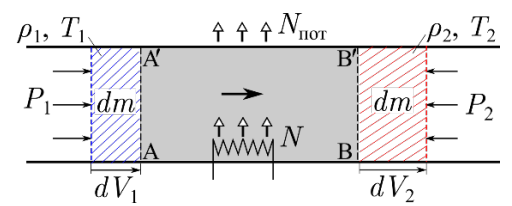
\includegraphics[scale=0.5]{foto2.png}
    \caption{Сдвиг фаз волны в трубе}
    \label{fig:sdvig}
\end{figure}\\
Теперь рассмотрим трубу, открытую на правом конце. Когда область сжатия достигнет открытого конца трубы, то у газа появится возможность распространяться во все стороны, в то время как в звуковой волне в трубе движение происходило только вдоль $x$. Поэтому область сжатия быстро рассасывается с увеличением расстояния от конца трубы, пока на некотором расстоянии (порядка радиуса трубы) давление не станет равным внешнему. Таким образом, если труба «подсоединена» к большой комнате, то на расстояниях от конца трубы порядка ее радиуса звуковое давление очень близко к нулю.\\
Пусть область сжатия достигла открытого конца. На открытом конце воздух вытекает из трубы и создает разрежение. Воздух на ближайшей к трубе части области разрежения испытывает меньшее сопротивление, чем «обычно», и стремится заполнить эту область, которая, таким образом, смещается влево. Воздух, примыкающий к сместившейся области разрежения, снова стремится вправо и т.д. Мы видим, что сжатие, перемещавшееся в направлении $+x$, вызвало разрежение, перемещающееся в направлении $-x$, что иллюстрирует рис.\ref{fig:sdvig}. Таким образом, в точке отражения за приходящим сжатием следует уходящее разрежение, и наоборот. Это значит, что на свободном конце трубы волна отражается, меняя свое направление на обратное.\\
При непрерывной работе источника волна, идущая от него будет складываться с отраженной волной. Считая, что отраженная волна имеет ту же амплитуду что и отраженная, записываем уравнения волны от источника $\xi_{1}$ и отраженной волны $\xi_{2}$ для открытой с одного конца трубы:
\begin{align}
    \xi_{1} &= A cos(\omega t - kx)\\
    \xi_{2} &= A cos(\omega t + kx)
\end{align}
В результате сложения колебание в точке $x$ будет происходить по закону:
\begin{equation}
    \xi = 2Asin(\omega t)sin(kx) = B(x)sin(\omega t).
\end{equation}
Получившаяся волна - стоячая. Точки, амплитуда колебаний которых равна нулю, называются узлами. Точки, колеблющиеся с максимальной амплитудой, называются пучностями.\\
Координаты узлов найдем из уравнения $B(x) = 0$ или $sin(kx) = 0$:\\
Это уравнение имеет решения:
\begin{equation}
    x = \frac{\pi n}{k} = \frac{n\lambda}{2}, n = 1,2,\ldots
\end{equation}\\
Из полученной формулы видно, что расстояние между соседними узлами равно половине длины волны.\\
На открытых концах давление воздуха равно атмосферному, то есть будут возникать узелы звукового давления и, следовательно, пучности смещения и скорости. Поэтому на длине трубы будет укладываться целое число длин полуволн.
\begin{align} \label{eq: dlina_voln}
    l &= n\frac{\lambda}{2}, n = 1,2,..\ldots\\
    \lambda_{n} &= \frac{2l}{n}, n = 1,2,\ldots
\end{align}\\
Длинам волн уравнения \ref{eq: dlina_voln} соответствуют частоты:
\begin{equation}
    \nu_{n} = \frac{c}{\lambda_{n}} = \frac{c\cdot n}{2l}
\end{equation}\\
Координаты пучностей найдем из уравнения $B(x) = \pm 1$ или $sin(kx) = \pm 1$:\\ 
\begin{equation}
    x = \left( n + \frac{1}{2} \right)\frac{\lambda}{2}, n = 1,2,\ldots
\end{equation}\\

\textbf{
Получаем, что частота будет:
\begin{equation}
    \nu_{n} =  \sqrt{\frac{\gamma R T}{M}}\frac{n}{2l}
\end{equation}
где $\gamma$ --- показатель адиабаты, $R$ --- универсальная газовая постоянная, $T$ --- температура воздуха, $M$ --- молярная масса воздуха, $l$ --- длина трубы, $n$ --- номер гармоники.
}
%====================================================================================================================================
\newpage
\subsection{Общее применение волновой теории для духовых инструментов}

Духовой музыкальный инструмент --- прибор, который издает звуки  определенных частоты, которые называются нотами, с помощью колебаний воздуха внутри себя. Есть разные духовые инструменты, и  у каждого свой способ возбуждения и усиления звуковых колебаний.

\begin{figure}[!ht]
    \centering
    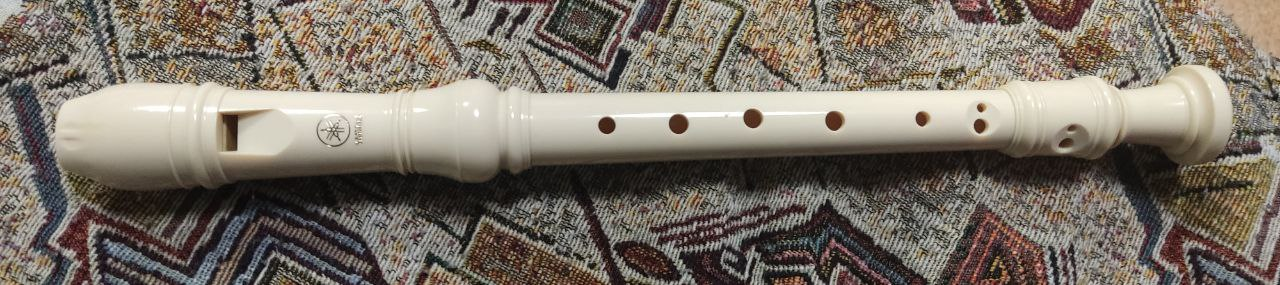
\includegraphics[scale=0.22]{block_1.jpg}
    \caption{Фото блок-флейты №1}
    \label{fig:foto_block_1}
\end{figure}
\begin{figure}[!ht]
    \centering
    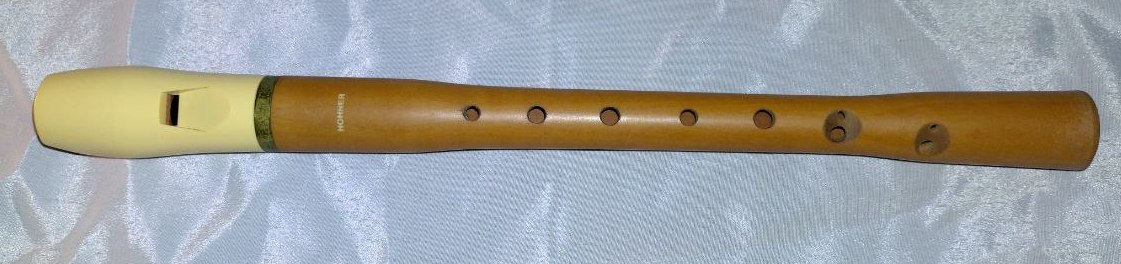
\includegraphics[scale=0.25]{block_2.jpg}
    \caption{Фото блок-флейты №2}
    \label{fig:foto_block_2}
\end{figure}
\begin{figure}[!ht]
    \centering
    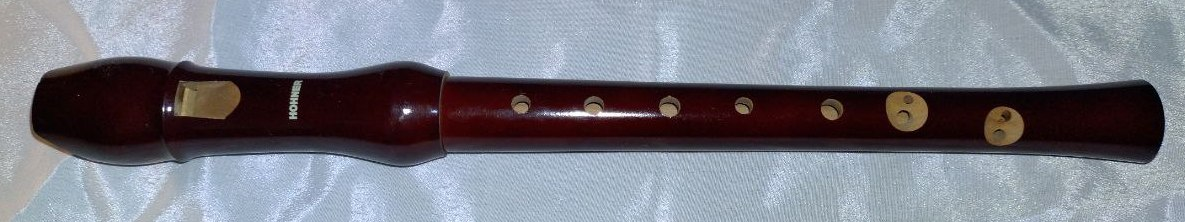
\includegraphics[scale=0.25]{block_3.jpg}
    \caption{Фото блок-флейты №3}
    \label{fig:foto_block_3}
\end{figure}
\begin{figure}[!ht]
    \centering
    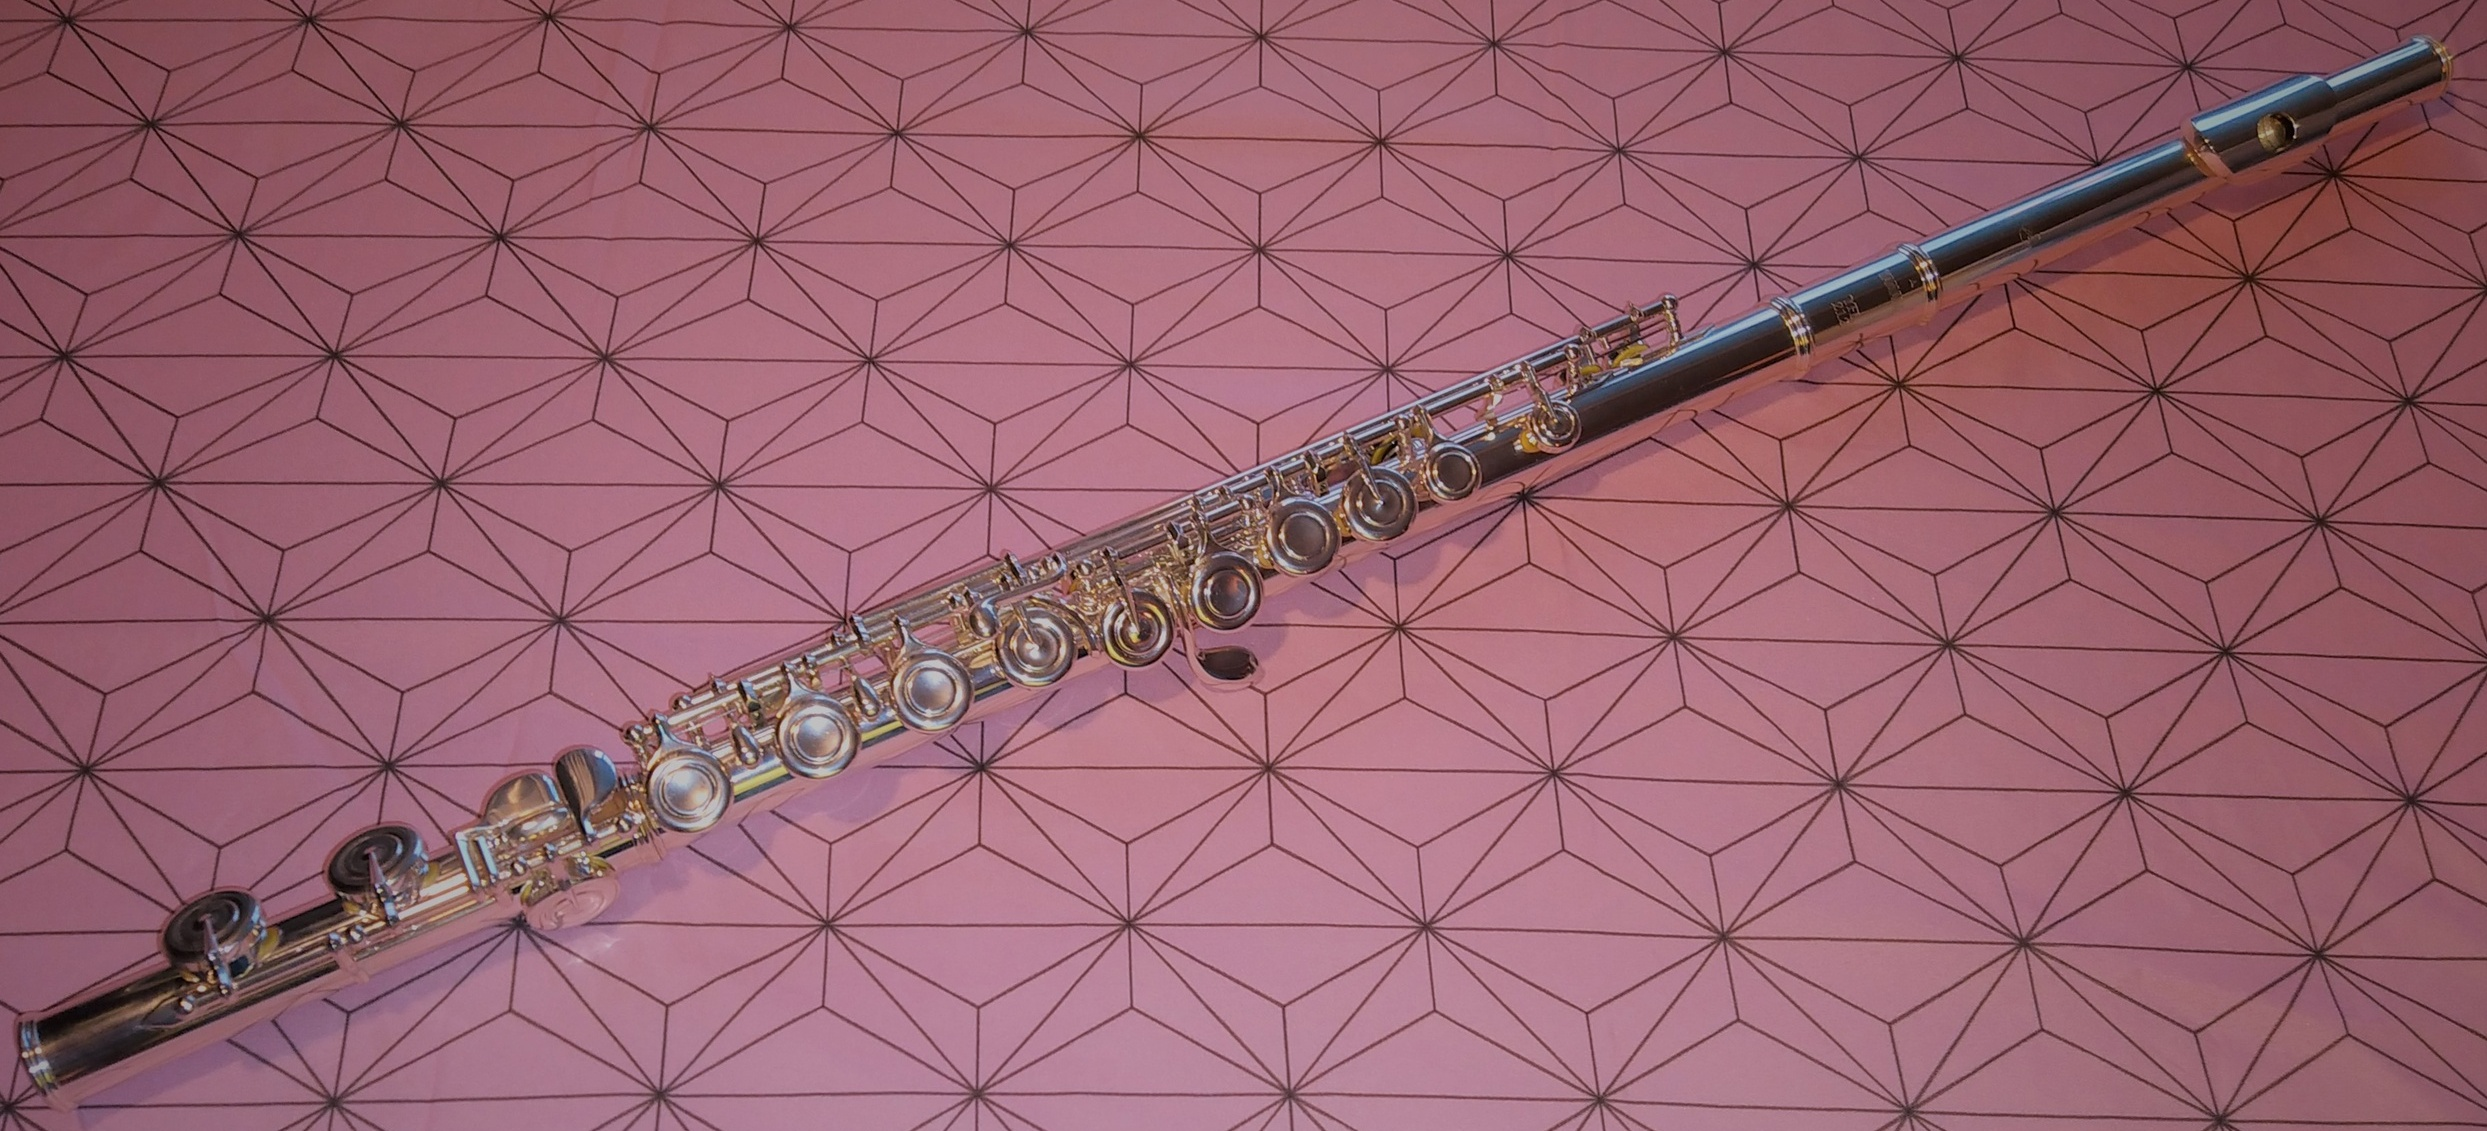
\includegraphics[scale=0.18]{big.jpg}
    \caption{Фото большой флейты}
    \label{fig:foto_big}
\end{figure}

В данной работе рассматриваются: поперечная(большая) флейта(рис.\ref{fig:foto_big}), которая возбуждает колебания через амбушюр и блок-флейта(рис.\ref{fig:foto_block_1},\ref{fig:foto_block_2},\ref{fig:foto_block_3}), которая возбуждает колебания через свисток. 

Мы рассматриваем эти инструменты как приближенную модель трубы с открытыми в атмосферу концами. в которых возбуждаются продольные стоячие волны. Для этого флейту считаем трубой, а расстояние отсчитывается от конца флейты(в случае большой) и от конца свистка(в случае блок-флейты) до первого открытого тонального отверстия.

Воздух,нагнетаемый источником, рассекается о свисток(рис.\ref{fig:razrez_blok_fleity}) или о стальной край амбушюра и затем создается два потока, один из которых создает давление в теле инструмента,за счет чего и начинаются колебания.

Они имеют разные особенности, и за счет этого можно изучить границы применимости приближений волновой теории.

На рис.\ref{fig:shema_volny_in_flute} и рис.\ref{fig:granichniy_sluchai} показано, как будет измеряться рабочая 
длина --- от начала колебаний --- амбушюра, до первого открытого отверстия.
\begin{figure}[!ht]
    \centering
    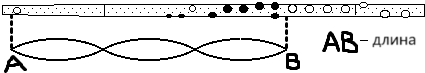
\includegraphics[scale=1]{fluteD6.png}
    \caption{Схема волны в флейте при одном открытом отверстии}
    \label{fig:shema_volny_in_flute}
\end{figure}
\begin{figure}[!ht]
    \centering
    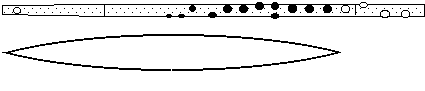
\includegraphics[scale=0.9]{fluteE.png}
    \caption{Граничный случай}
    \label{fig:granichniy_sluchai}
\end{figure}
Для всех инструментов существует общая музыкальная теория, согласно которой они должны излучать одинаковые 
частоты --- ноты. Существует четкое соответствие между нотами и соответствующим им нотам --- таблица \ref{tab:zavisimost_not}.

%===================================================================================================================================
\subsection{Устройство флейты}

Рассмотрим устройство классической флейты (рис.\ref{fig:classical_fleita} и рис.\ref{fig:applicatyra_classical_fleita})

Особенности:
\begin{enumerate}
    \item В сечении --- цилиндр с фиксированным диаметром
    \item Все отверстия рассматриваемых аппликатур имеют одинаковый диаметр.
    \item Открыта с обоих концом(амбушюр и другой конец)
\end{enumerate}

\begin{figure}[!ht]
    \centering
    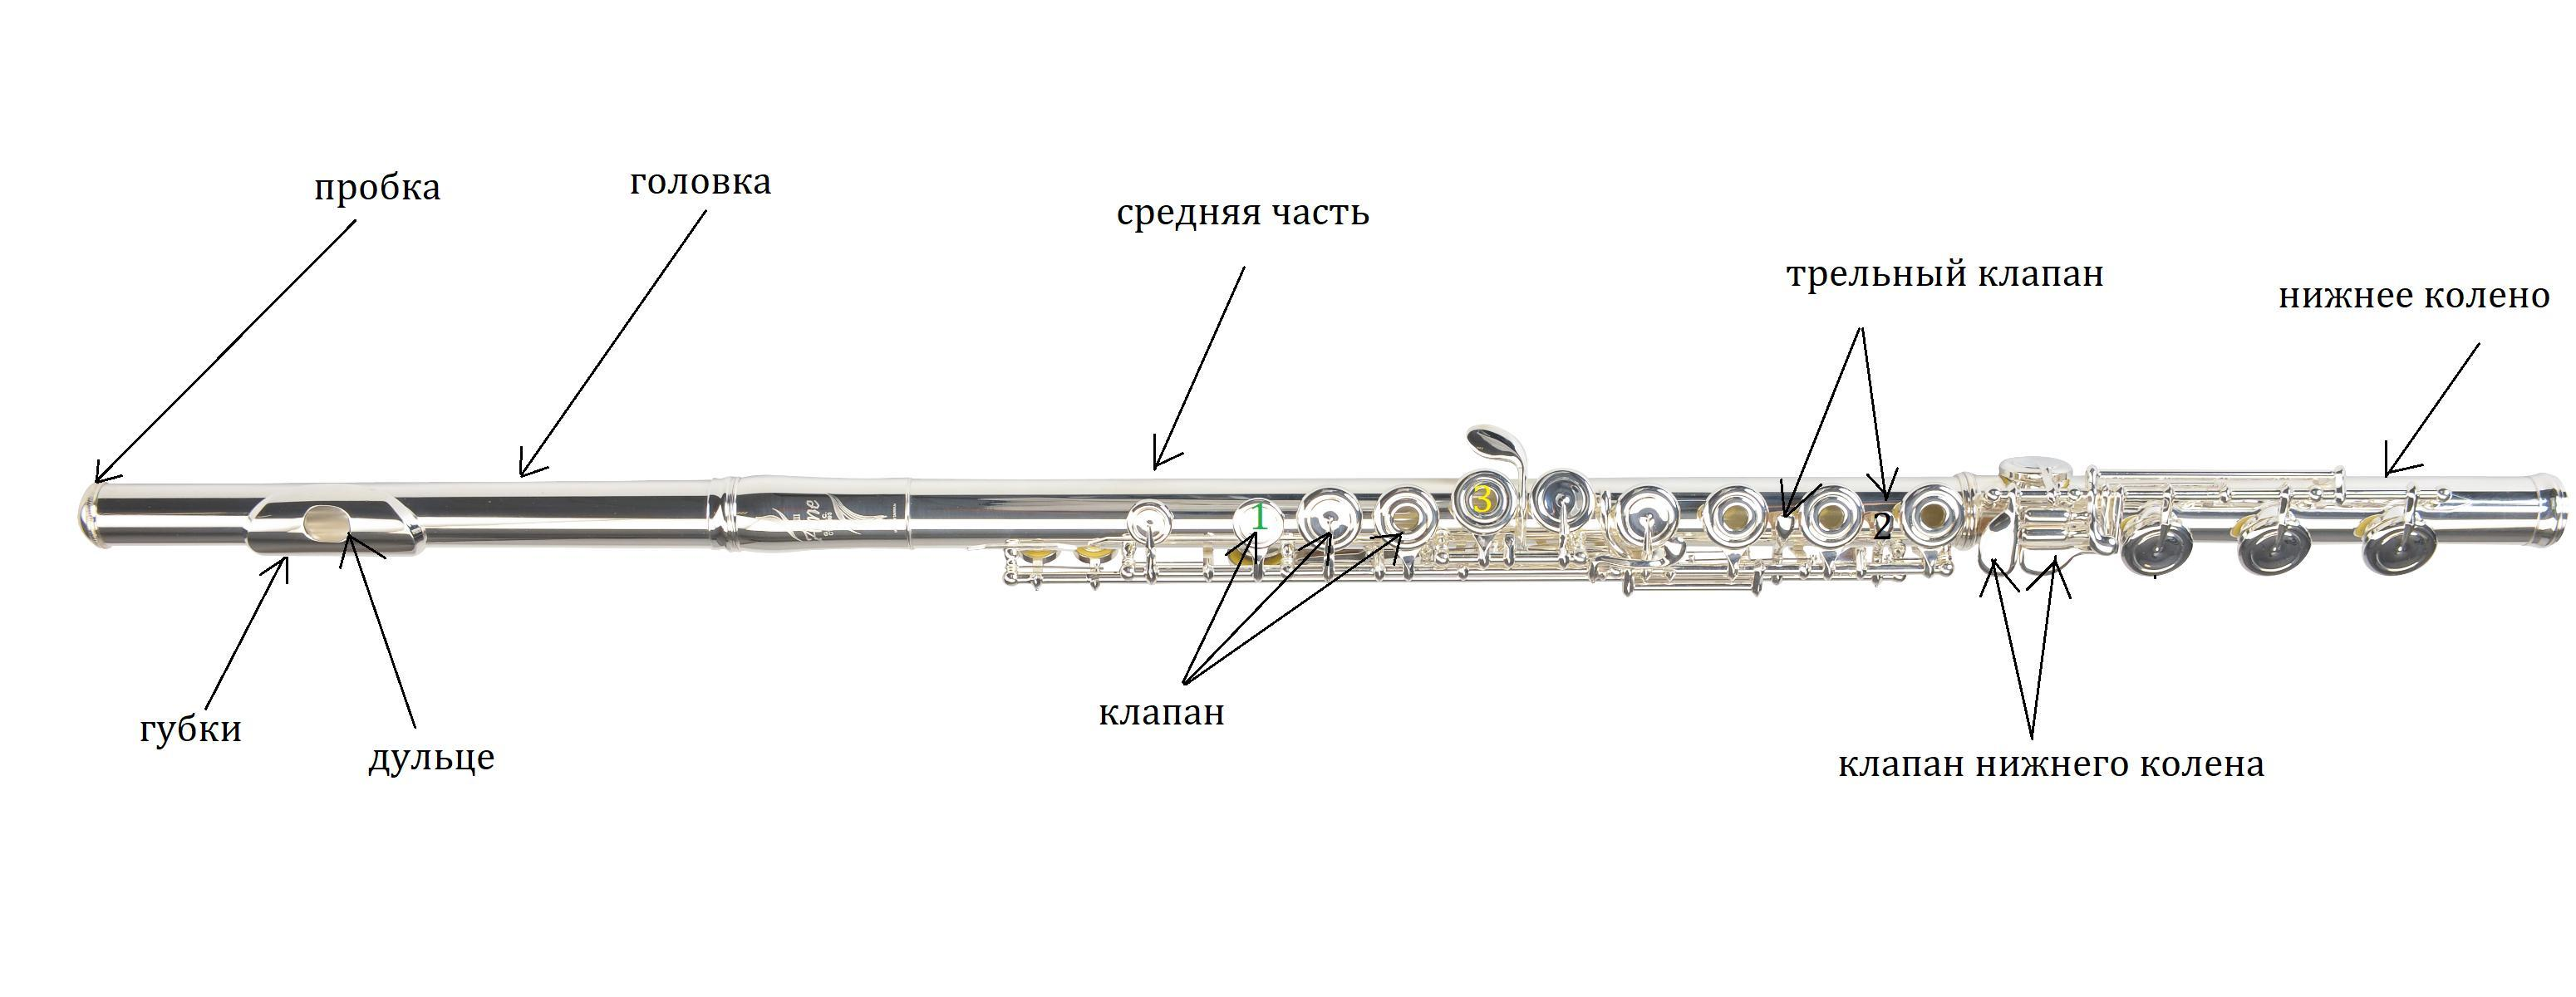
\includegraphics[scale=0.23]{foto8.jpg}
    \caption{Устройство классической флейты}
    \label{fig:classical_fleita}
\end{figure}
\begin{figure}[!ht]
    \centering
    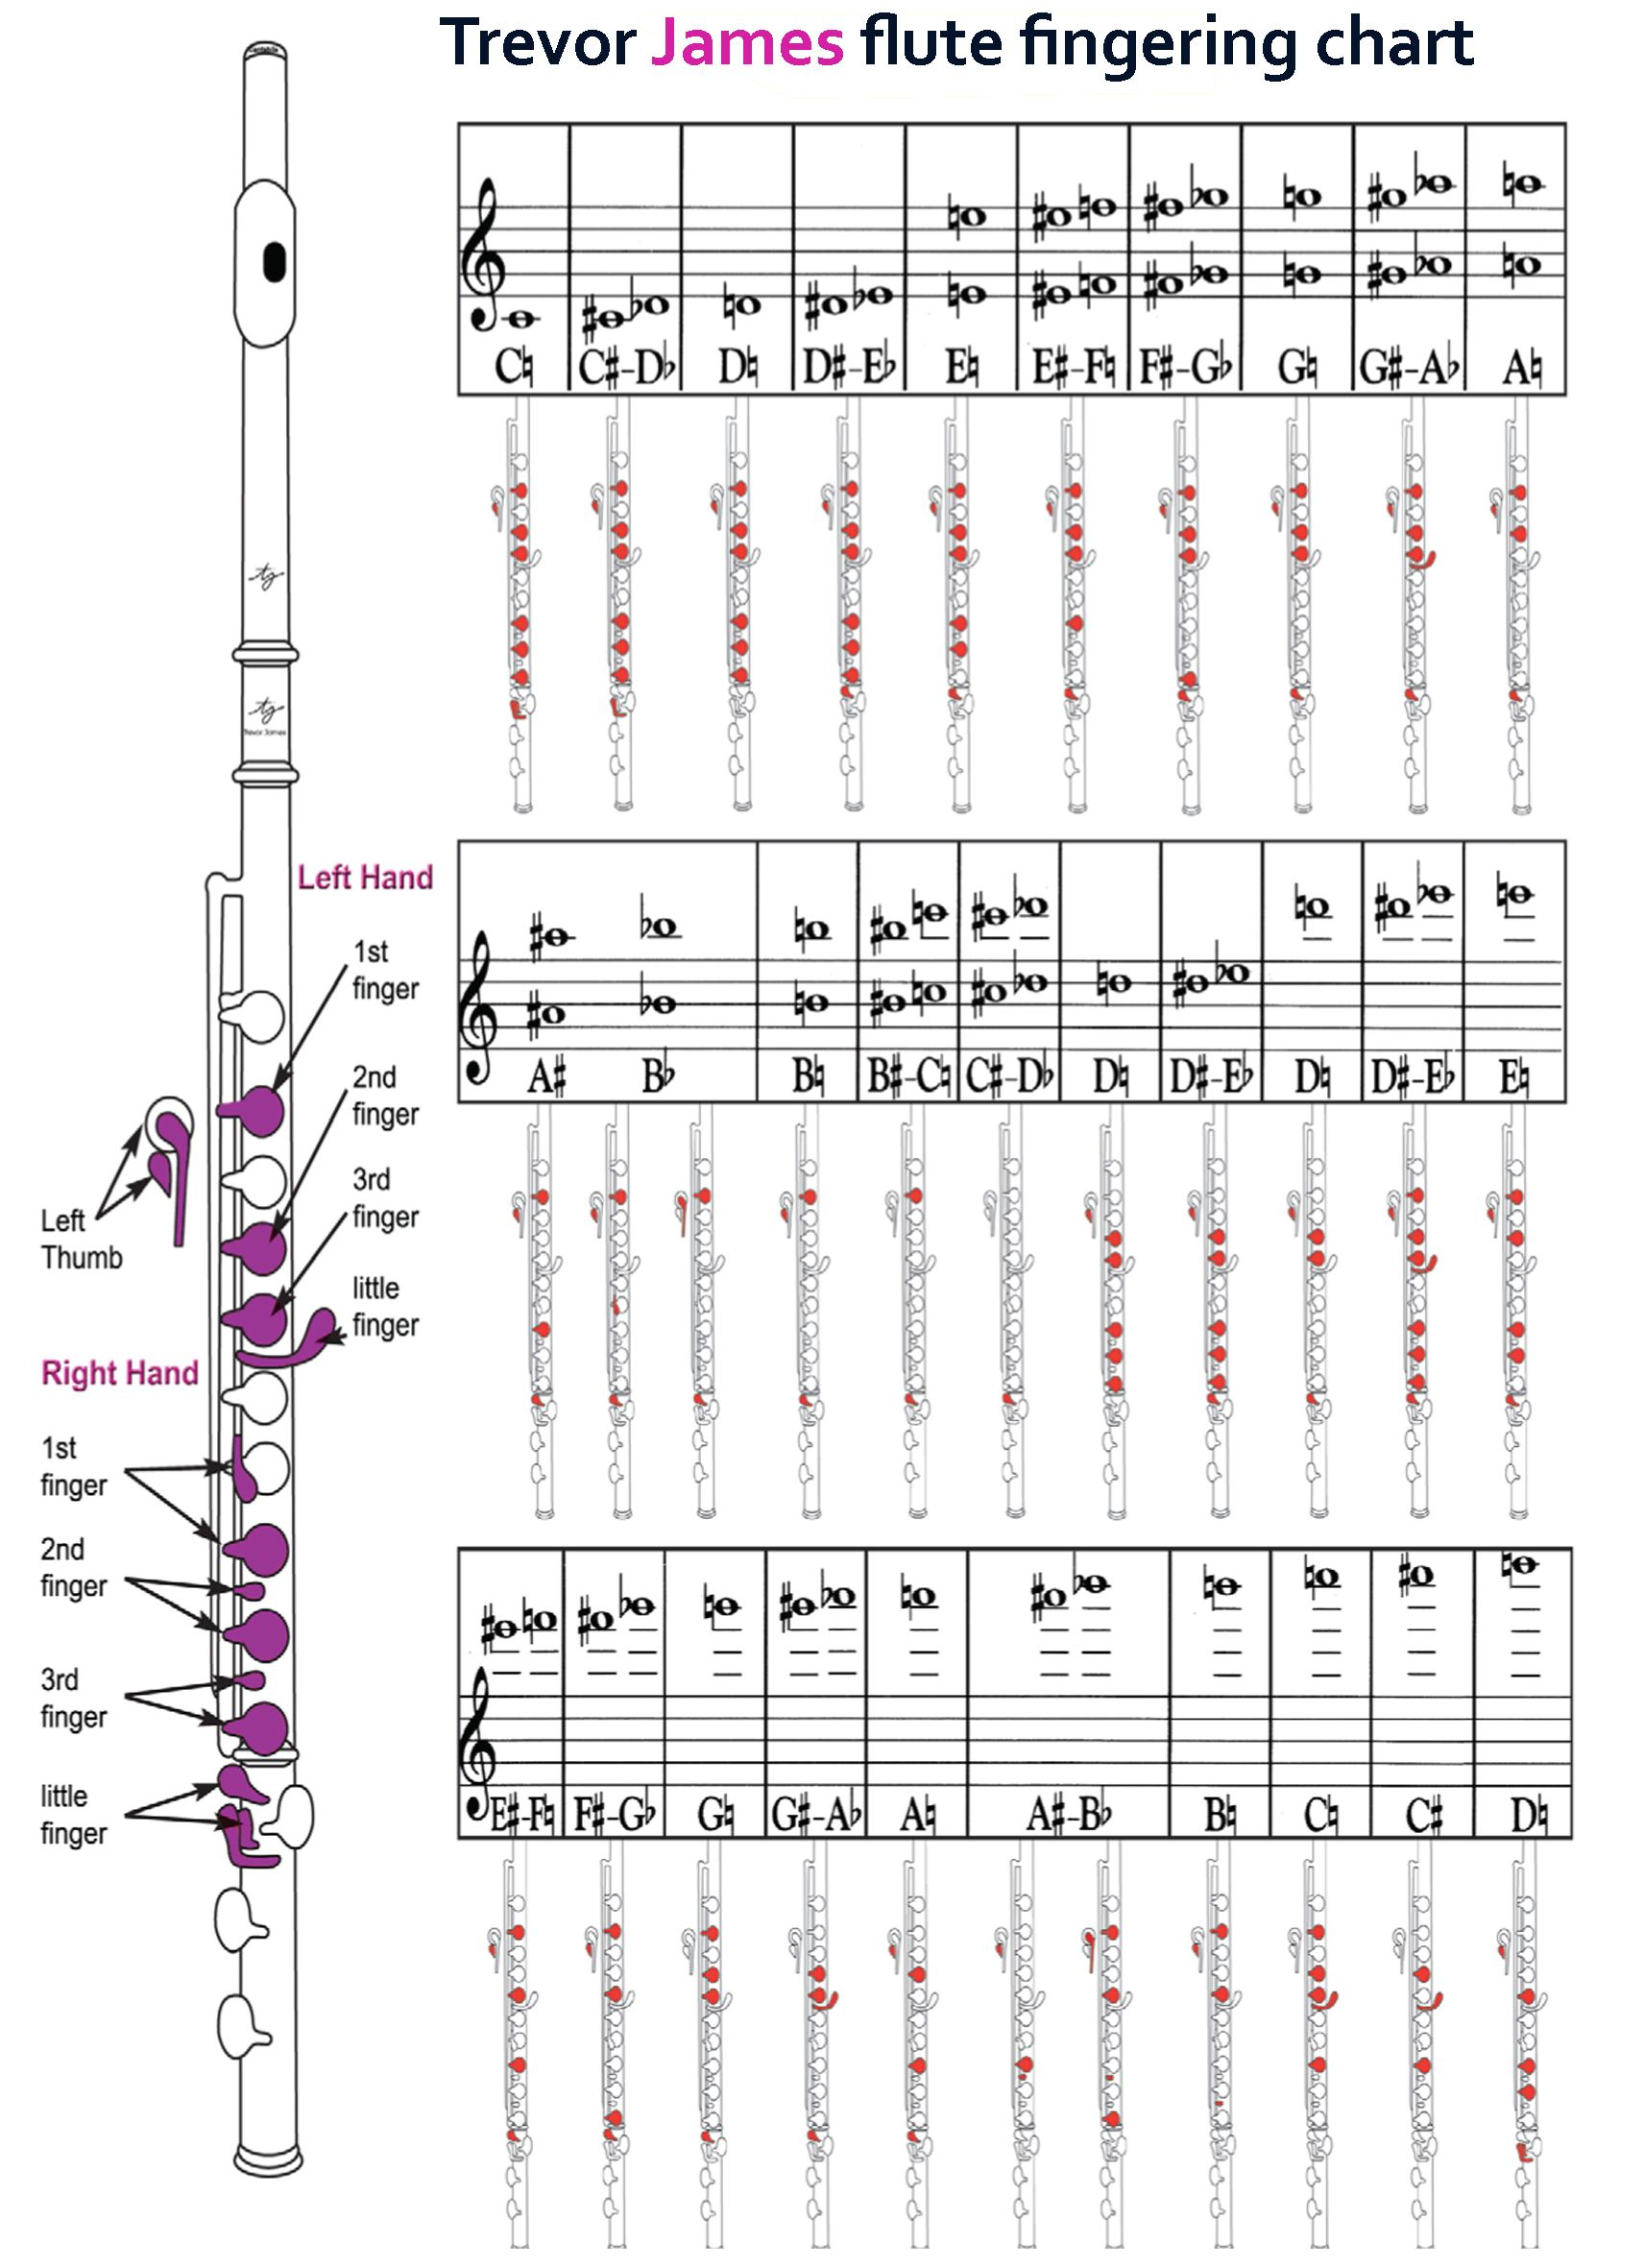
\includegraphics[scale=0.47]{foto9.jpg}
    \caption{Аппликатура классической флейты}
    \label{fig:applicatyra_classical_fleita}
\end{figure}

Из-за этих особенностей классическая флейта является очень близким к идеальному прибором для проверки волновой теории --- колебания воздуха в трубе.

\subsection{Устройство блок-флейты}

Рассмотрим устройство блок-флейты (рис.\ref{fig:razrez_blok_fleity} и рис.\ref{fig:applikatura_blok_fleity}):
\begin{figure}[!ht]
    \centering
    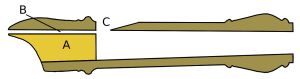
\includegraphics[scale=0.74]{foto4.png}
    \caption{Разрез блок-флейты}
    \label{fig:razrez_blok_fleity}
\end{figure}

\begin{figure}[!ht]
    \centering
    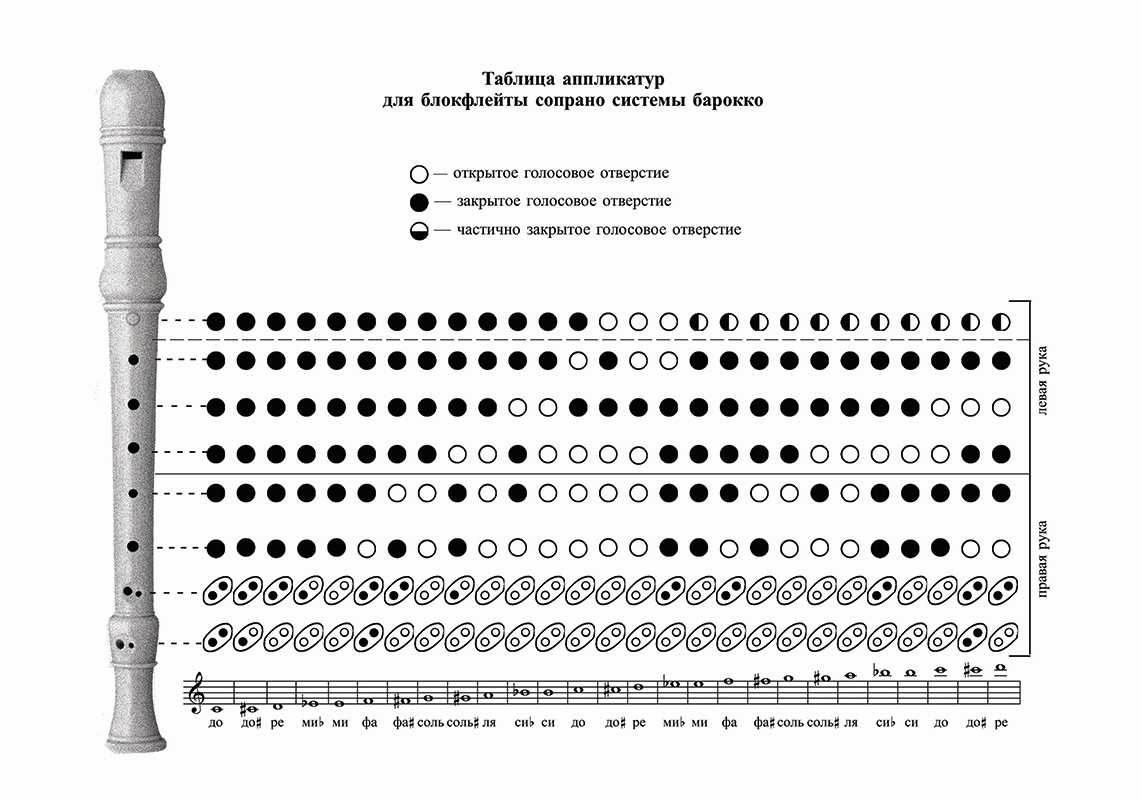
\includegraphics[scale=0.74]{foto3.jpg}
    \caption{Аппликатура блок-флейты}
    \label{fig:applikatura_blok_fleity}
\end{figure}

Особенности:
\begin{enumerate}
    \item В отличии от классической флейты блок-флейта имеет свисток.
    \item Отверстия имеют разный диаметр, а также расположены на разном расстоянии друг от друга.
    \item Ее внутреннее пространство --- усеченный конус в отличии от классической цилиндрической флейты.
\end{enumerate}

Из-за этих особенностей строения нужно учитывать, что на блок-флейту можно применять теорию колебаний воздуха 
в трубе, но как показал эксперимент с большими поправками. 

%TODO: hoboy

%===========================================================================================================================
\newpage

\section{Результаты эксперимента}

Эксперимент заключался в измерении частот звуков, извлекаемых из духовых инструментов, и длин.

С помощью микрофона и анализатора частот, были зарегистрированы ноты и их частоты при разных гармониках.
Результаты представлены в таблицах, сам эксперимент показан на рис.\ref{fig:postanovka_experimenta_blok_fleita}

Далее обработав запись, были сняты частоты для разных гармоник --- рис.\ref{fig:primer_dannih}

Снятые данные для блок флейты 1,2,3 --- 1 столбец таблицы ~\ref{tab:dannie_dla_blok_fleita_1},~\ref{tab:dannie_dla_blok_fleita_2},~\ref{tab:dannie_dla_blok_fleita_3}

Снятые данные для большой флейты --- 1 столбец таблицы ~\ref{tab:dannie_dla_big_fleita}

\newpage

\section{Обработка результатов}

Воспользуемся зависимостью частоты колебаний воздуха в трубке, выведенные ранее:
\begin{equation}
    v_{\text{зв}} = \sqrt{\frac{\gamma R T}{M}}\approx 347.8\frac{\text{м}}{\text{с}}
\end{equation}
где $\gamma = 1.4$, $R = 8.31 \frac{\text{Дж}}{\text{моль}\cdot\text{К}}$, $T = 28.5^\circ C\text{(температура внутри флейты с погрешностью}0.1^\circ C)$, $M = 29 \frac{\text{г}}{\text{моль}}$, 

\begin{equation}
    l_{\text{эф}} = \frac{\lambda}{2} = \frac{v_{\text{зв}}}{2\nu}
\end{equation}
где $l_{\text{эф}}$ --- эффективная длина рабочей части инструмента

\begin{equation}
    \nu(n,l) = 347.8\frac{n}{2l}
\end{equation}

После применения этих зависимостей можно рассчитать эффективную и реальную длину, а также снятую и расчетную частоту.

Для блок-флейты 1,2,3 --- таблицы ~\ref{tab:dannie_dla_blok_fleita_1},~\ref{tab:dannie_dla_blok_fleita_2},~\ref{tab:dannie_dla_blok_fleita_3}

Для большой флейты --- таблица ~\ref{tab:dannie_dla_big_fleita}

По этим данным построим график реальной длины от обратной частоты $l_{real} = a + k \cdot \frac{1}{\nu}$, 
для проверки корректности использования уравнения колебаний для духового инструмента, используя аппроксимацию МНК.

Для блок-флейты 1,2,3 --- рис.\ref{fig:graphic_block_1_real},\ref{fig:graphic_block_2_real},\ref{fig:graphic_block_3_real}.

Для большой флейты --- рис.\ref{fig:graphic_big_real}.

Расчет погрешности при аппроксимации по МНК:
\[k = \frac{\langle xy\rangle-\langle x\rangle \langle y\rangle}{\langle x^2\rangle - \langle x\rangle^2}\]
\[\sigma_{k} = \frac{1}{\sqrt{N-2}}\sqrt{\frac{\langle y^2 \rangle - \langle y \rangle ^2}{\langle x^2 \rangle - \langle x \rangle ^2} - k^2}\]
\[b = \langle y \rangle - k \langle x\rangle \]
\[\sigma_{b} = \sigma_{k} \cdot \sqrt{\langle x^2 \rangle}\]
Систематические погрешности:
\begin{itemize}
    \item При измерении длины инструментальная погрешность 0.5 мм.
    \item При измерении температуры $0.1^\circ C$.
    \item При измерении частоты погрешность микрофона 1 Гц.
\end{itemize}
\newpage
Для графика зависимости реальной длины от обратной частоты, таблица \ref{tab:data_graphics}

\begin{table}[!ht]
\centering
\begin{tabular}{|c|c|c|c|c|}
\hline
             & Блок-флейта №1                   & Блок-флейта №2                    & Блок-флейта №3                   & Большая флейта                    \\ \hline
             & $l_{real}$                       & $l_{real}$                        & $l_{real}$                       & $l_{real}$                        \\ \hline
$k$          & 182.39    & 181.50   & 179.83  & 172.01   \\ \hline
$b$          & -0.061 & -0.0705 & -0.064 & -0.0025 \\ \hline
$\sigma_{k}$ & 11.08                            & 5.02                              & 5.62                             & 0.308                             \\ \hline
$\sigma_{b}$ & 0.015                            & 0.0073                            & 0.0082                           & 0.00089                           \\ \hline
\end{tabular}
    \caption{Данные снятые с графиков и их погрешности}
    \label{tab:data_graphics}
\end{table}

Коэффициент наклона $k = \frac{v_{\text{зв}}}{2}$ поэтому можно узнать реальную скорость звука в флейте: $v_{\text{1}} = 364.6 \frac{\text{м}}{\text{с}}, v_{\text{2}} = 363\frac{\text{м}}{\text{с}}, v_{\text{3}} = 359,6 \frac{\text{м}}{\text{с}},v_{\text{4}} = 344 \frac{\text{м}}{\text{с}}$

Сравним данные полученные из графиков:
\begin{itemize}
    \item Все зависимости линейны(в пределах погрешностей), что показывает применимость волновой теории на духовые инструменты
    \item В изучении большой флейты имеет место: высокая точность между коэффициентами наклона, незначительная погрешность. Значит расчетная с использованием волновой теории скорость звука точно совпала с реальной. Низкая погрешность означает что устройство большой флейты идеально
    \item В изучении блок-флейты(1,2,3) имеет место: график имеет свободный член и более высокий угол наклона, более высокая погрешность. Это объясняется тем что наша модель приближенная и зависит от многих факторов. Положение узлов не точно совпадает с положением отверстий, а зависит от многих параметров вплоть до диаметра сечения, размеры свистка. Эти поправки определяются чаще всего эмперическим способом. Подробнее написано в работе Пауля Диккенса по моделированию флеты.
\end{itemize}

%=============================================================================================================================
\newpage
\section{Выводы}
В работе были исследованы колебания воздуха в трубе и изучена применимость волновой теории к духовым инструментам. Проведя серию экспериментов, были собраны данные для 4 инструментов, 3 блок-флейты и 1 большая флейты.
Обработка данных показала, что волновая теория очень точно ложится на большую флейту, из-за ее строения близкого к идеальной трубе. Также обработка показала, что волновая теория плохо ложится на блок-флейту из-за ее неидельного строения, усеченный конус с разными расстояниями до отверстий.

%=============================================================================================================================
\newpage
\section{Приложение}
\subsection{Таблицы}
Для основных тонов: до, ре, ми, фа, соль, ля, си разных октав можно получить разные частоты. Но существует общая таблица перевода из нот в частоты.
\begin{table}[!ht]
    \centering
    \begin{tabular}{|c|c|c|c|c|c|c|c|c|c|}
    \hline
           & \textbf{Контр} & \textbf{Большая} & \textbf{Малая} & \textbf{Первая} & \textbf{Вторая} & \textbf{Третья} & \textbf{Четвертая} & \textbf{Пятая} \\ \hline
           & 1              & 2                & 3              & 4               & 5               & 6               & 7                  & 8              \\ \hline
    До     & 32,7           & 65,4             & 130,8          & 261,6           & 523,2           & 1046,50         & 2093,00            & 4186           \\ \hline
    Ре     & 36,7           & 73,4             & 146,8          & 293,6           & 587,3           & 1174,7          & 2349,3             & 4698,6         \\ \hline
    Ми     & 41,2           & 82,4             & 164,8          & 329,6           & 659,2           & 1318,5          & 2637               & 5274           \\ \hline
    Фа     & 43,6           & 87,3             & 174,6          & 349,2           & 698,4           & 1396,9          & 2793,8             & 5587,6         \\ \hline
    Соль   & 49             & 98               & 196            & 392             & 784             & 1568            & 3135,9             & 6271,9         \\ \hline
    Ля     & 55             & 110              & 220            & 440             & 880             & 1760            & 3520               & 7040           \\ \hline
    Си     & 61,7           & 123,4            & 246,9          & 493,8           & 987,7           & 1975,5          & 3951,1             & 7902,1         \\ \hline
    \end{tabular}
    \caption{Табличная зависимость частоты от ноты по октавам}
    \label{tab:zavisimost_not}
\end{table}

\begin{table}[!ht]
    \centering
    \begin{tabular}{|c|c|c|c|}
    \hline
    Нота & Снятые частоты,Гц & Эффективная длина,м & Реальная длина,м    \\ \hline
    До   & 535                & 0,322                & 0,28              \\ \hline
    Ре   & 592                & 0,29                 & 0,237             \\ \hline
    Ми   & 668                & 0,258                & 0,23              \\ \hline
    Фа   & 705                & 0,244                & 0,193             \\ \hline
    Соль & 785                & 0,219                & 0,167             \\ \hline
    Ля   & 889                & 0,194                & 0,145             \\ \hline
    Си   & 979                & 0,176                & 0,123             \\ \hline
    \end{tabular}
    \caption{Данные для блок-флейты №1}
    \label{tab:dannie_dla_blok_fleita_1}
\end{table}

\begin{table}[!ht]
    \centering
    \begin{tabular}{|c|c|c|c|}
    \hline
    Нота & Снятые частоты, Гц & Эффективная длина, м & Реальная длина, см \\ \hline
    До   & 521                & 0,331                & 28,4               \\ \hline
    Ре   & 586                & 0,294                & 23,3               \\ \hline
    Ми   & 662                & 0,260                & 20,4               \\ \hline
    Фа   & 697                & 0,247                & 18,5               \\ \hline
    Соль & 785                & 0,219                & 16,2               \\ \hline
    Ля   & 879                & 0,196                & 13,8               \\ \hline
    Си   & 990                & 0,174                & 11,4               \\ \hline
    \end{tabular}
    \caption{Данные для блок-флейты №2}
    \label{tab:dannie_dla_blok_fleita_2}
\end{table}

\begin{table}[!ht]
    \centering
    \begin{tabular}{|c|c|c|c|}
    \hline
    Нота & Снятые частоты, Гц & Эффективная длина, м & Реальная длина, см \\ \hline
    До   & 527                & 0,327                & 28,3               \\ \hline
    Ре   & 586                & 0,294                & 23,6               \\ \hline
    Ми   & 662                & 0,260                & 20,8               \\ \hline
    Фа   & 697                & 0,247                & 18,7               \\ \hline
    Соль & 785                & 0,219                & 16,4               \\ \hline
    Ля   & 879                & 0,196                & 14,2               \\ \hline
    Си   & 984                & 0,175                & 12                 \\ \hline
    \end{tabular}
    \caption{Данные для блок-флейты №3}
    \label{tab:dannie_dla_blok_fleita_3}
\end{table}

\begin{table}[!ht]
    \centering
    \begin{tabular}{|c|c|c|c|}
    \hline
    Нота   & Снятые частоты,Гц & Эффективная длина,см & Реальная длина,см \\ \hline
    До     & 521                & 67                   & 65,7             \\ \hline
    До\#   & 551                & 62,9                 & 61,7             \\ \hline
    Ре     & 586                & 59,7                 & 58,4             \\ \hline
    Ре\#   & 621                & 56,3                 & 55               \\ \hline
    Ми     & 656                & 53,2                 & 52               \\ \hline
    Фа     & 697                & 50,1                 & 49               \\ \hline
    Фа\#   & 738                & 47,4                 & 46,4             \\ \hline
    Соль   & 785                & 44,6                 & 43,6             \\ \hline
    Соль\# & 832                & 42,3                 & 41,2             \\ \hline
    Ля     & 879                & 39,8                 & 38,9             \\ \hline
    Ля\#   & 938                & 37,6                 & 36,7             \\ \hline
    Си     & 990                & 35,4                 & 34,6             \\ \hline
    \end{tabular}
    \caption{Данные сдвига длин для большой флейты}
    \label{tab:dannie_dla_big_fleita}
\end{table}
%==============================================================================================================================
\subsection{Фотографии}
\newpage
\begin{figure}[!p]
    \centering
    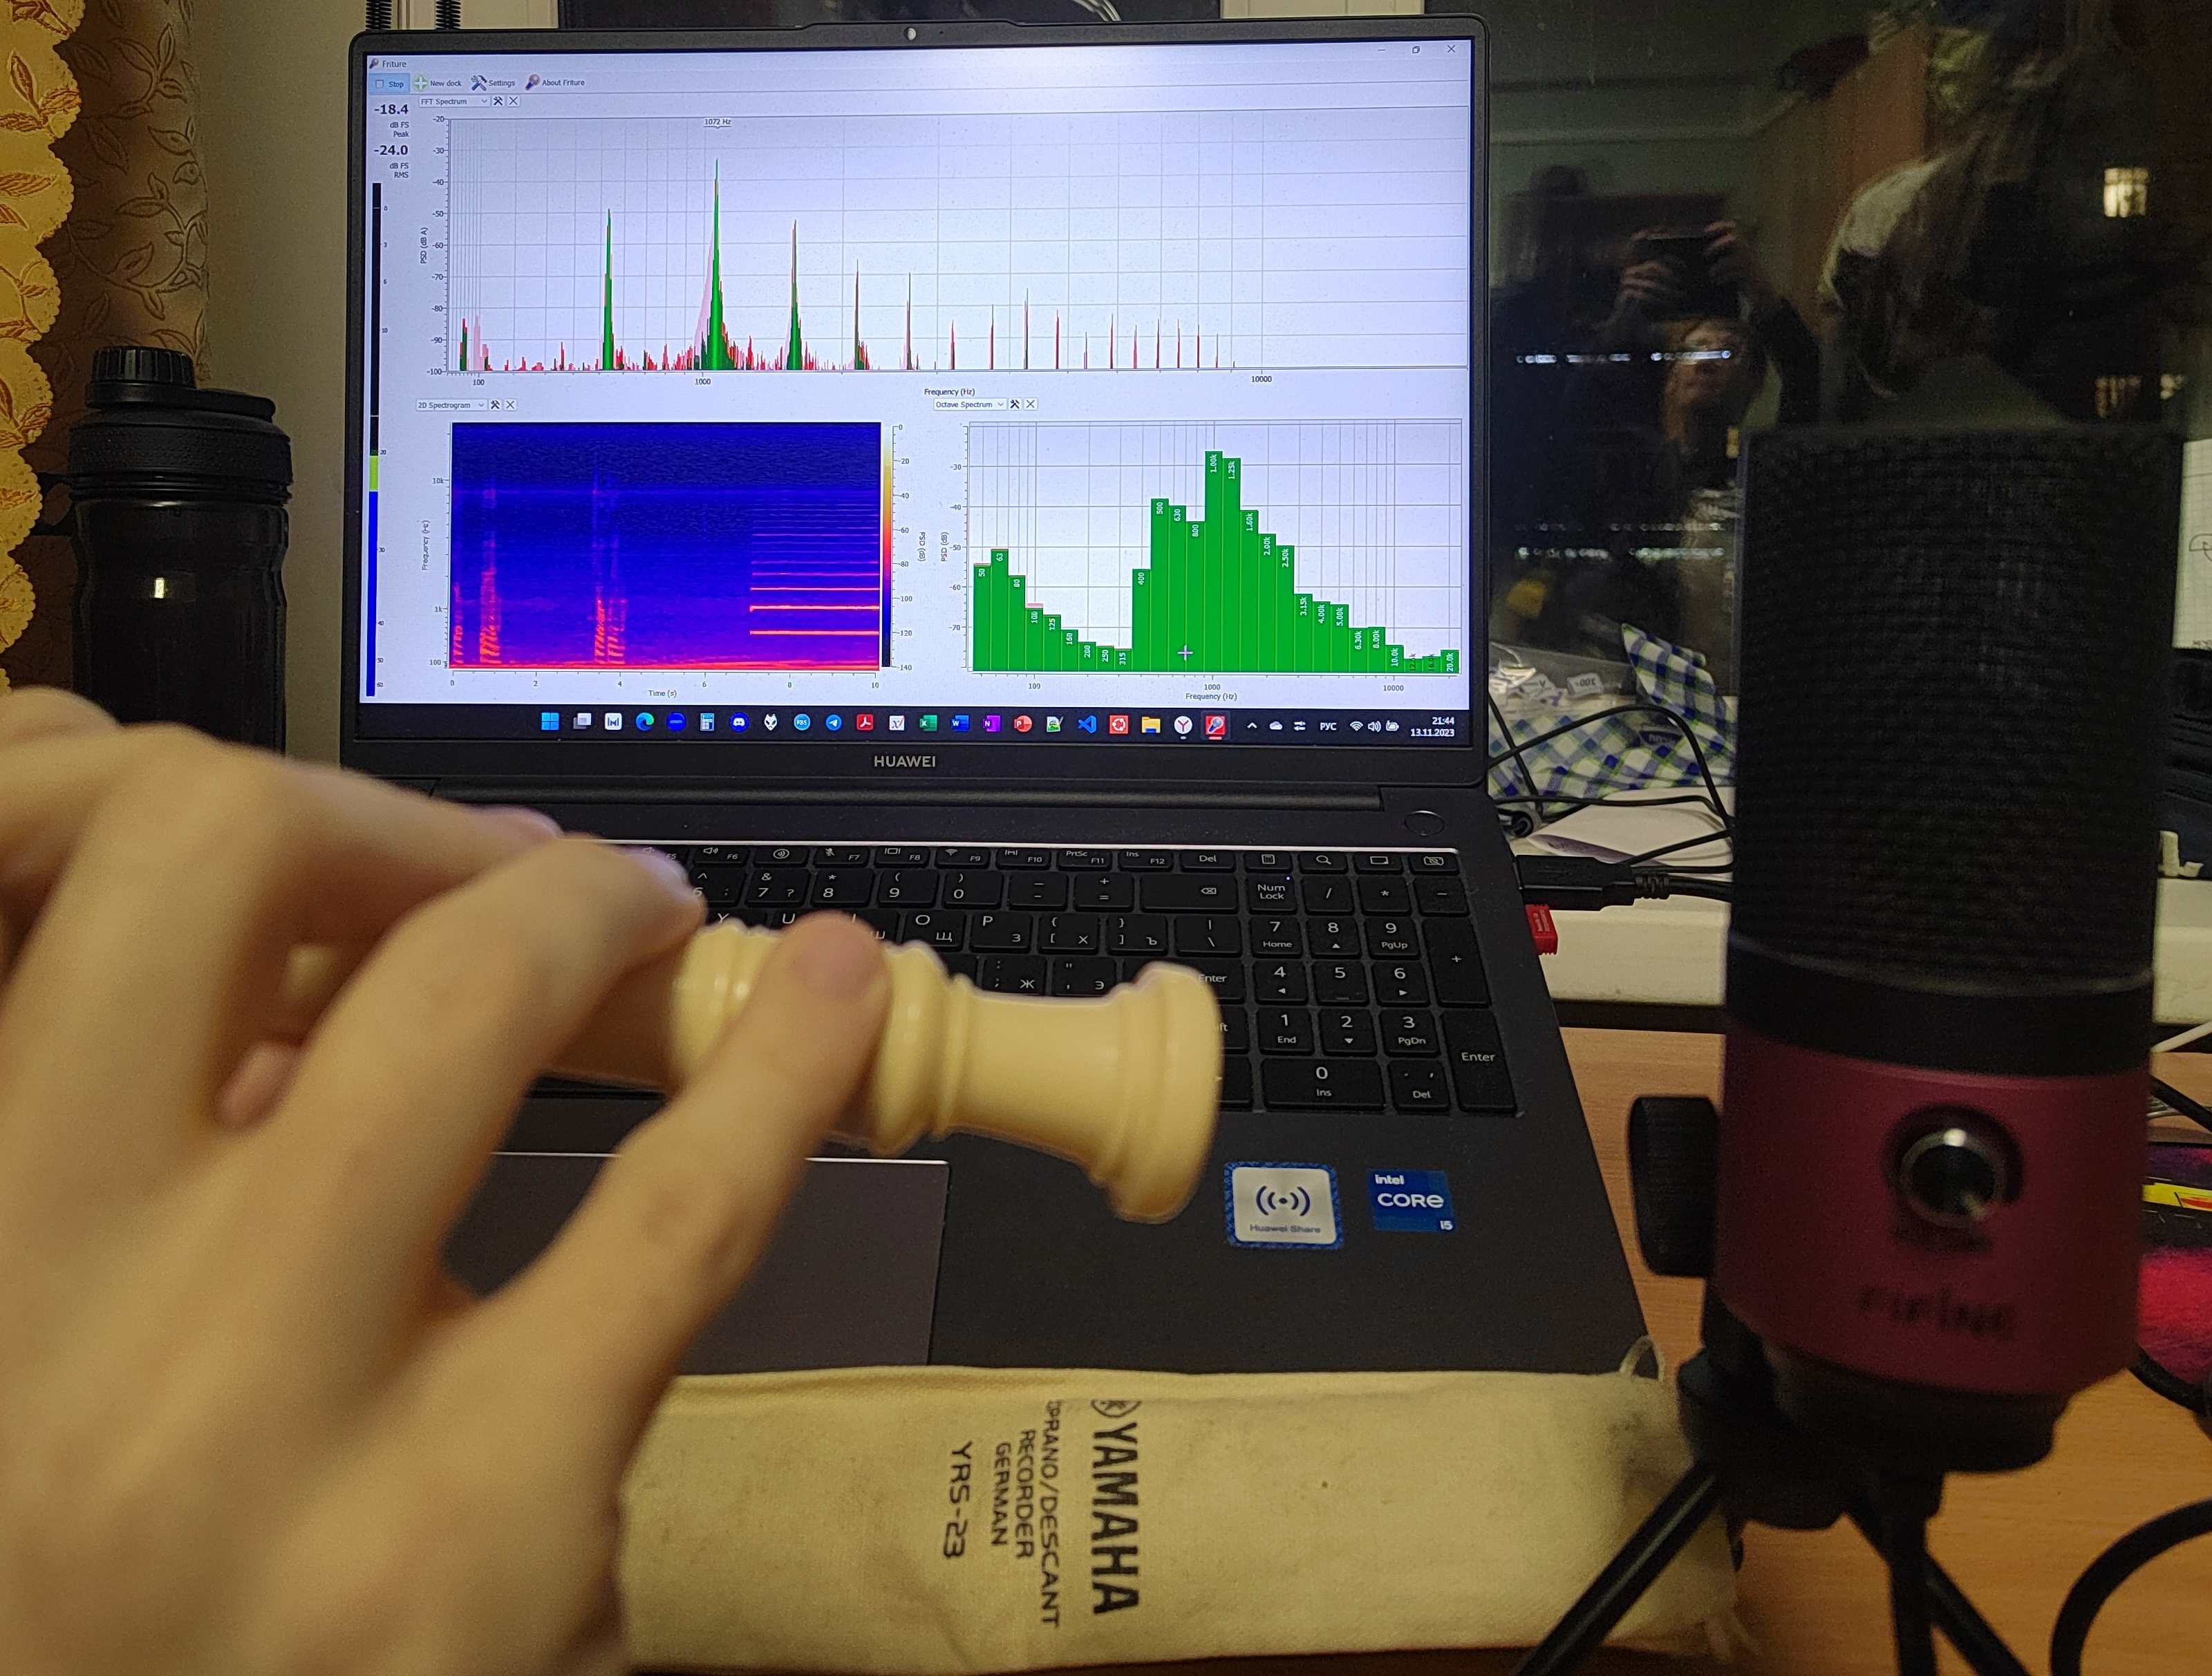
\includegraphics[scale=0.15]{foto5.jpg}
    \caption{Постановка эксперимента(блок-флейта)}
    \label{fig:postanovka_experimenta_blok_fleita}
\end{figure}

\newpage
\begin{figure}[!p]
    \centering
    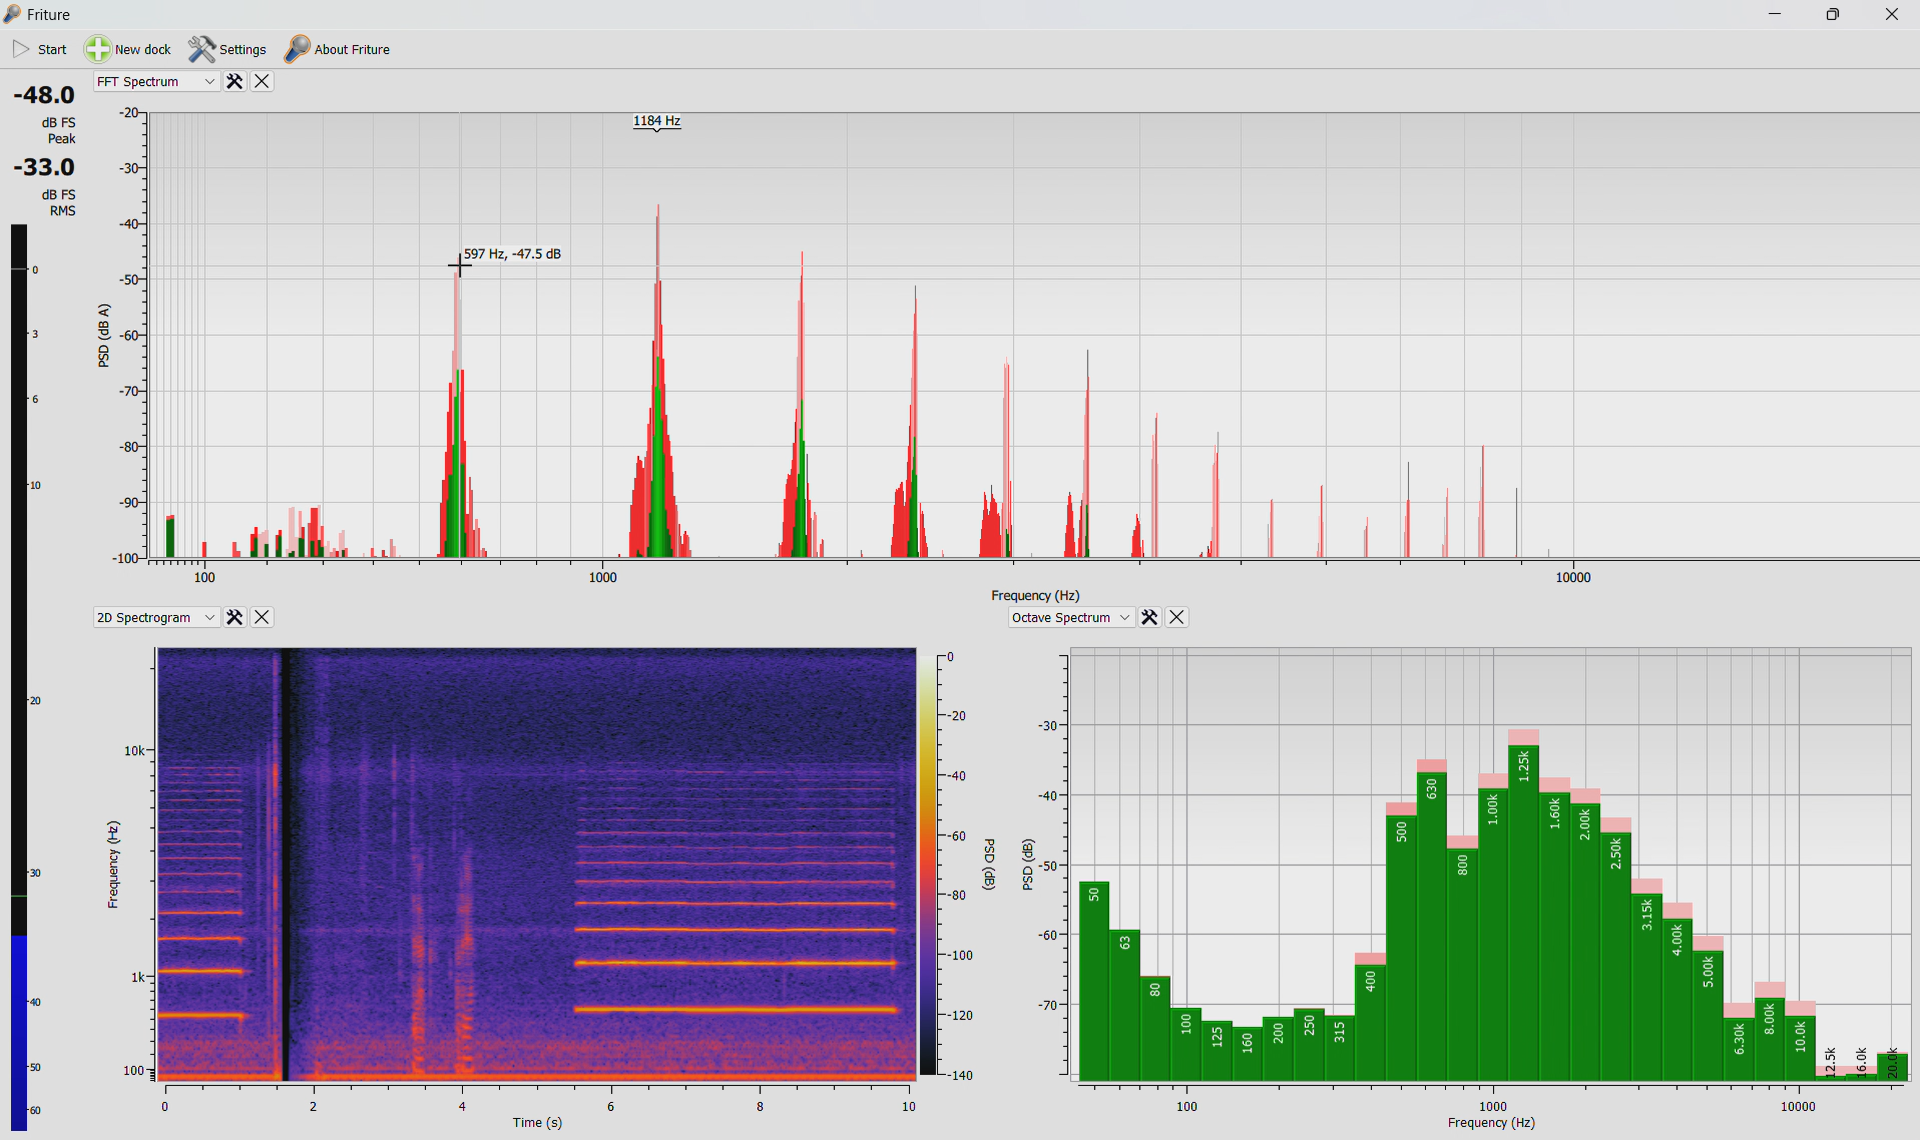
\includegraphics[scale=0.27]{data1.png}
    \caption{Пример данных полученных в эксперименте}
    \label{fig:primer_dannih}
\end{figure}

\newpage
\begin{figure}[!p]
    \centering
    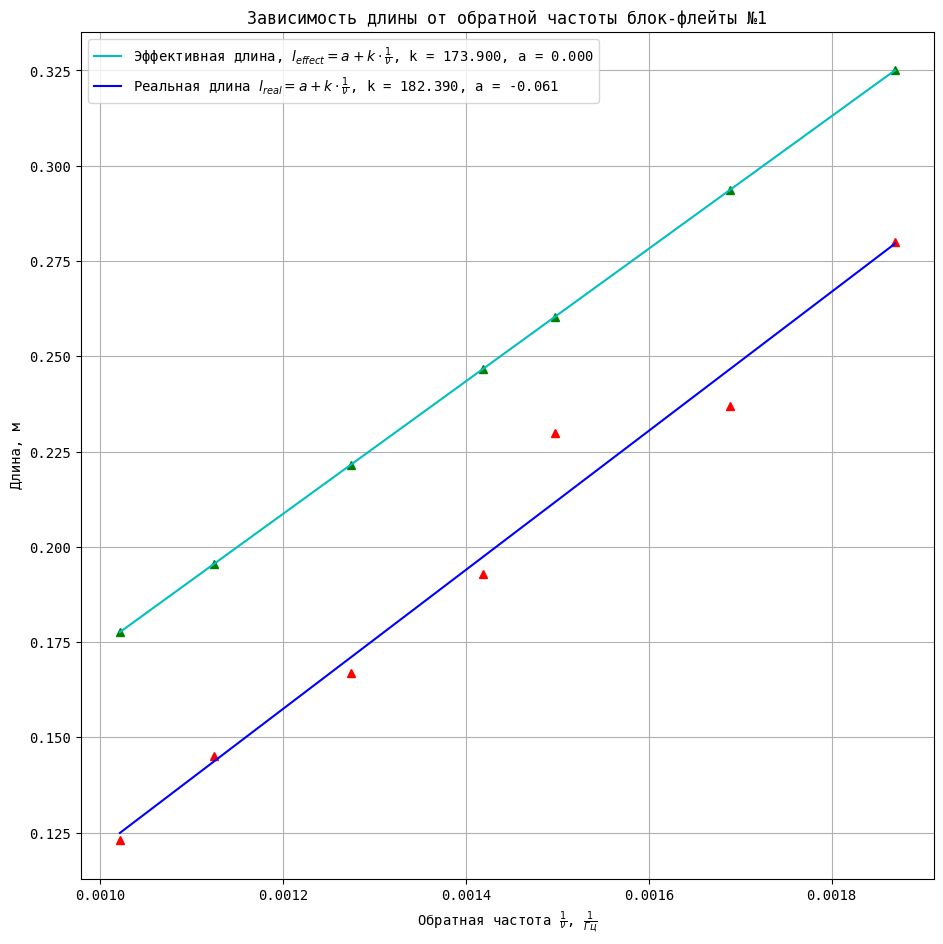
\includegraphics[scale=0.74]{graphic_block_1_full.png}
    \caption{График зависимости реальной длины от обратной частоты для блок-флейты №1}
    \label{fig:graphic_block_1_real}
\end{figure}

\newpage
\begin{figure}[!p]
    \centering
    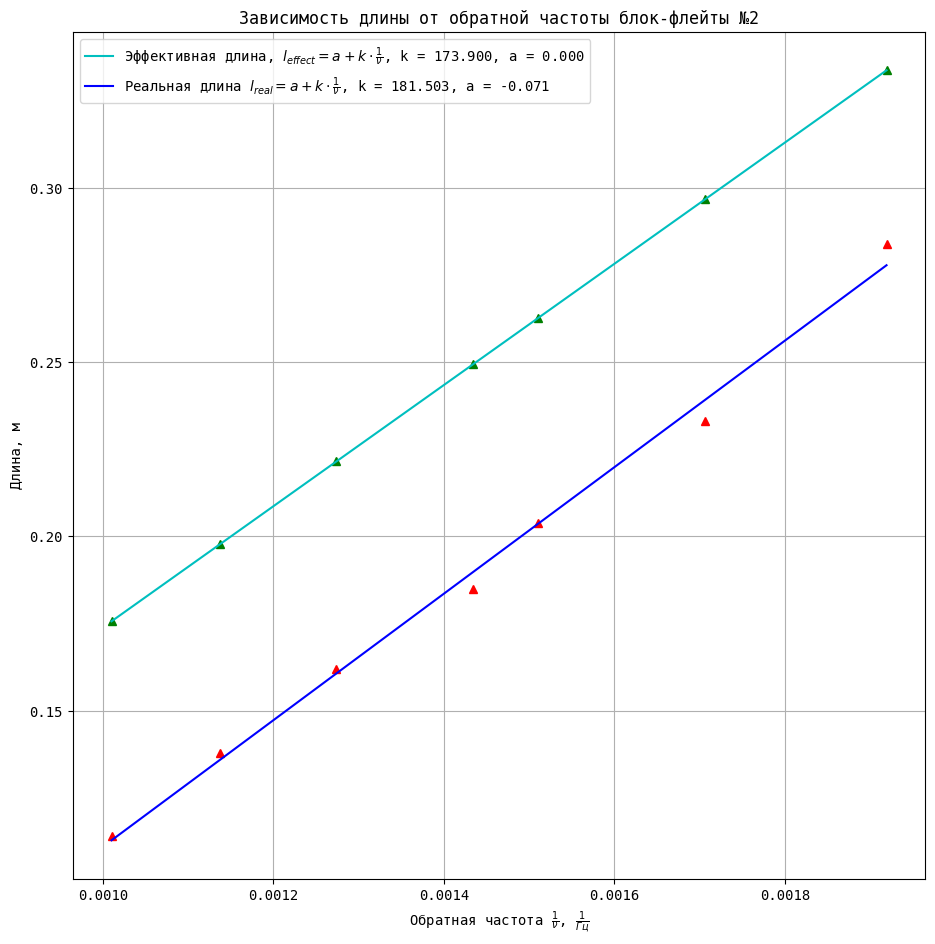
\includegraphics[scale=0.74]{graphic_block_2_full.png}
    \caption{График зависимости реальной длины от обратной частоты для блок-флейты №2}
    \label{fig:graphic_block_2_real}
\end{figure}

\newpage
\begin{figure}[!p]
    \centering
    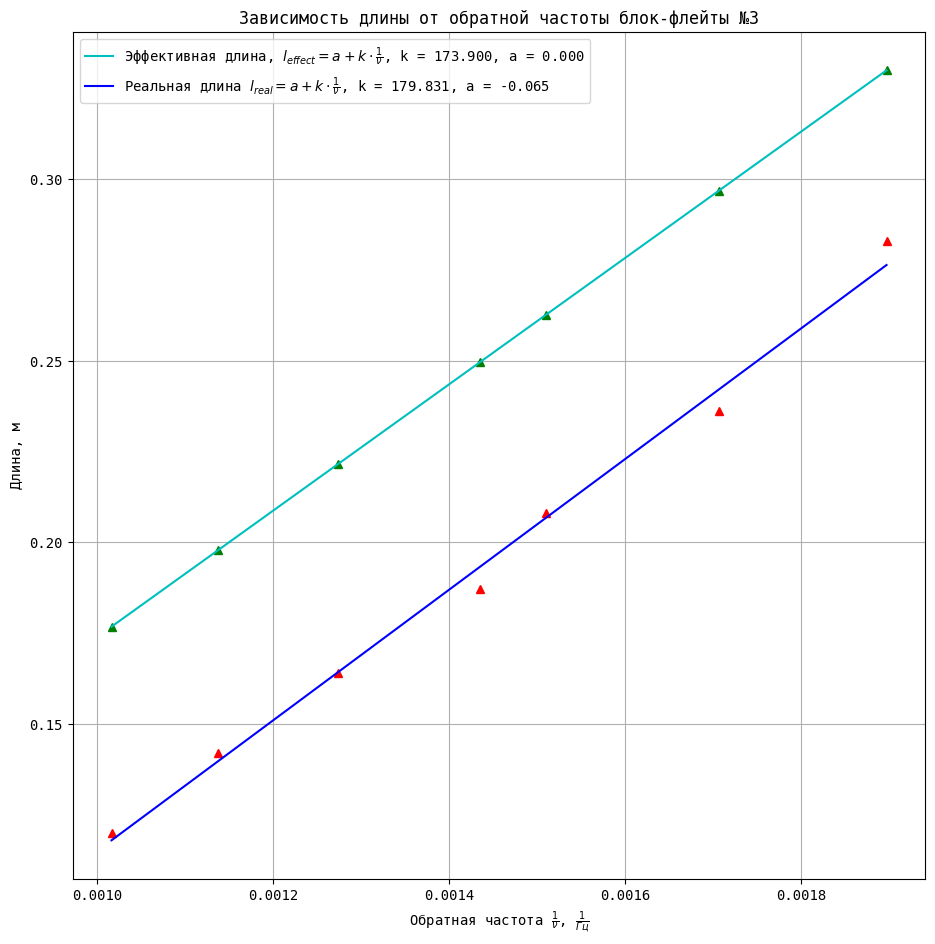
\includegraphics[scale=0.74]{graphic_block_3_full.png}
    \caption{График зависимости реальной длины от обратной частоты для блок-флейты №3}
    \label{fig:graphic_block_3_real}
\end{figure}

\newpage
\begin{figure}[!p]
    \centering
    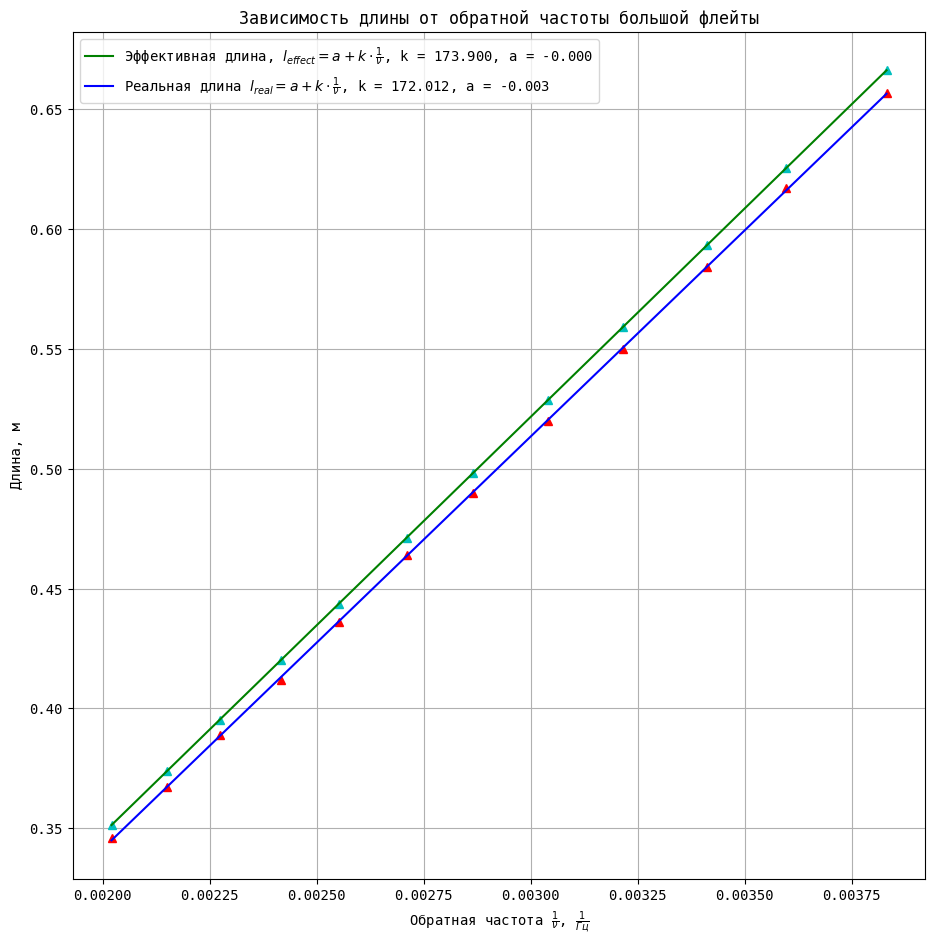
\includegraphics[scale=0.74]{graphic_big_full.png}
    \caption{График зависимости реальной длины от обратной частоты для большой флейты}
    \label{fig:graphic_big_real}
\end{figure}
%==============================================================================================================
\newpage
\newpage
\section{Источники}

\begin{enumerate}
    \item \href{https://newt.phys.unsw.edu.au/jw/fluteacoustics.html}{Flute acoustics: an introduction to how a flute works(сайт)}
    \item \href{https://ru.wikipedia.org/wiki/Равномерно_темперированный_строй}{Равномерно темперированный строй(сайт)}
    \item Ландау Л.Д., Лифшиц Е.М. Гидродинамика, 350 стр.
    \item Paul Dickens. Flute acoustics: measurement, modelling and design. 2007 г.
\end{enumerate}